
\section{Motores}  \label{secao_motores}

\subsection{Motores DC}


Um motor DC é essencialmente uma máquina elétrica de corrente contínua, que
converte energia elétrica de corrente contínua em energia mecânica. Máquinas
elétricas de corrente contínua são mais fácies de se controlar (quando
comparadas a máquinas de corrente alternada) e oferecem uma grande faixa de
velocidades \cite{Maquinas_eletricas}. Devido a essas características, tornam-se
boas candidatas para uso em eletrônica e robótica, uma vez que é viável
utilizá-las com com baterias. Para controlar a velocidade de um motor, é
necessário o uso de um encoder, que converte o sinal de posição em um valor
mensurável de velocidade angular, e também um driver, que permite a
microcontroladores controlarem a atuação do motor.

\subsubsection{Encoder magnético}

	Encoders magnéticos são um tipo de encoder rotacional que utiliza sensores 
	para identificar alterações em campos magnéticos a partir de uma roda ou 
	anel magnéticos. A rotação detectada é expressa em termos de pulsos de maior
	ou menor duração, a depender da resolução do encoder. Um encoder incremental
	mede a posição relativa do eixo (em contraste com encoders absolutos), em
	incrementos, a partir de dois sensores magnéticos, indicando a quantidade de
	pulsos percorridos entre a posição de referência e a posição atual.
	
	Há alguns tipos diferentes de se medir e representar a resolução de um
	encoder magnético. Na representação de pulsos por revolução (PPR), o valor 
	apresentado descreve o número de pulsos em valor alto que um encoder terá em
	qualquer uma das suas duas saídas quadráticas. Uma outra representação comum
	de resolução de encoders é CPR (contagens por revolução), que representa o
	número de estados de quadratura decodificados que existem entre as duas
	saídas do encoder (representando, portanto, o valor de uma resolução dada em
	PPR multiplicada por 4). Outras formas de representar a resolução de um
	encoder são LPR (linhas por revolução, referindo-se a às barras marcadas no
	disco óptico de um encoder, cada uma representando um pulso de valor baixo),
	e também ciclos por revolução (cujo acrônimo ocasionalmente é dado também
	como CPR por fabricantes) - o valor apresentado em ambas as representações 
	equivale à representação em PPR (que é a representação adotada para
	avaliação e apresentação dos componentes utilizados neste trabalho). 
	
	Em encoders magnéticos incrementais, são produzidas duas ondas quadradas
	como saídas, A e B \cite{encoder_ppr}. As duas possuem 90° de fase entre si,
	e, caso a onda A esteja adiantada em relação a B (\autoref{encoder_ppr_ab}),
	o sentido de rotação é positivo (anti-horário).

\begin{figure}[ht]
	\centering
	\caption{Encoder holzer}
	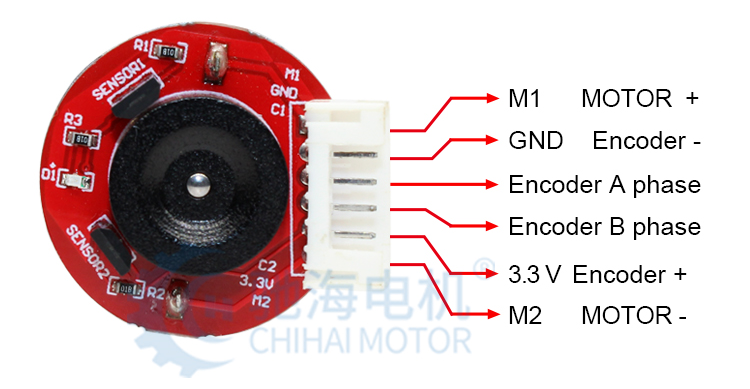
\includegraphics[width=0.6\textwidth]{figures/encoder_holzer}
	\caption{FONTE: \cite{motor_dc_6v_encoder}}
\end{figure}

\begin{figure}[ht]
	\centering
	\caption{Ondas quadradas resultantes dos pulsos de saída do encoder}
	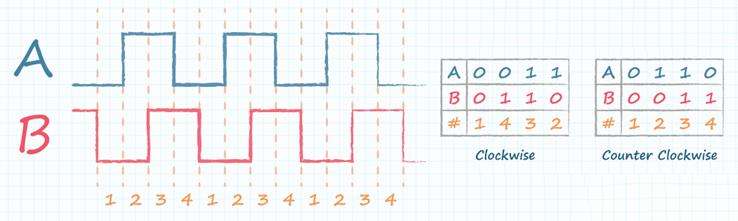
\includegraphics[width=0.6\textwidth]{figures/encoder_pulso_ab}
	\caption{FONTE: \cite{encoder_ppr}}
	\label{encoder_ppr_ab}
\end{figure}


\subsubsection{Motor DC e encoder}
Para a versão inicial do robô, foi decidido trabalhar com motor DC.
Motores DC são mais difíceis de controlar que motores de passo, porém tem uma resposta mais rápida, e se o controle for
bem aplicado, podem ter também um melhor desempenho. A complexidade do controle de um motor DC apresenta um bom desafio
para aplicação dos conceitos e disciplinas do curso de Engenharia de Instrumental, Automação e Robótica. O motor DC 
escolhido foi um de 6V 210rpm, com taxa de redução de 1:34. Tal motor já possui um encoder magnético acoplado, com 11
PPR (\textit{"Pulses Per Revolution"}), resultando em um encoder com resolução de 374 PPR.

\begin{figure}[htb]
	\centering
	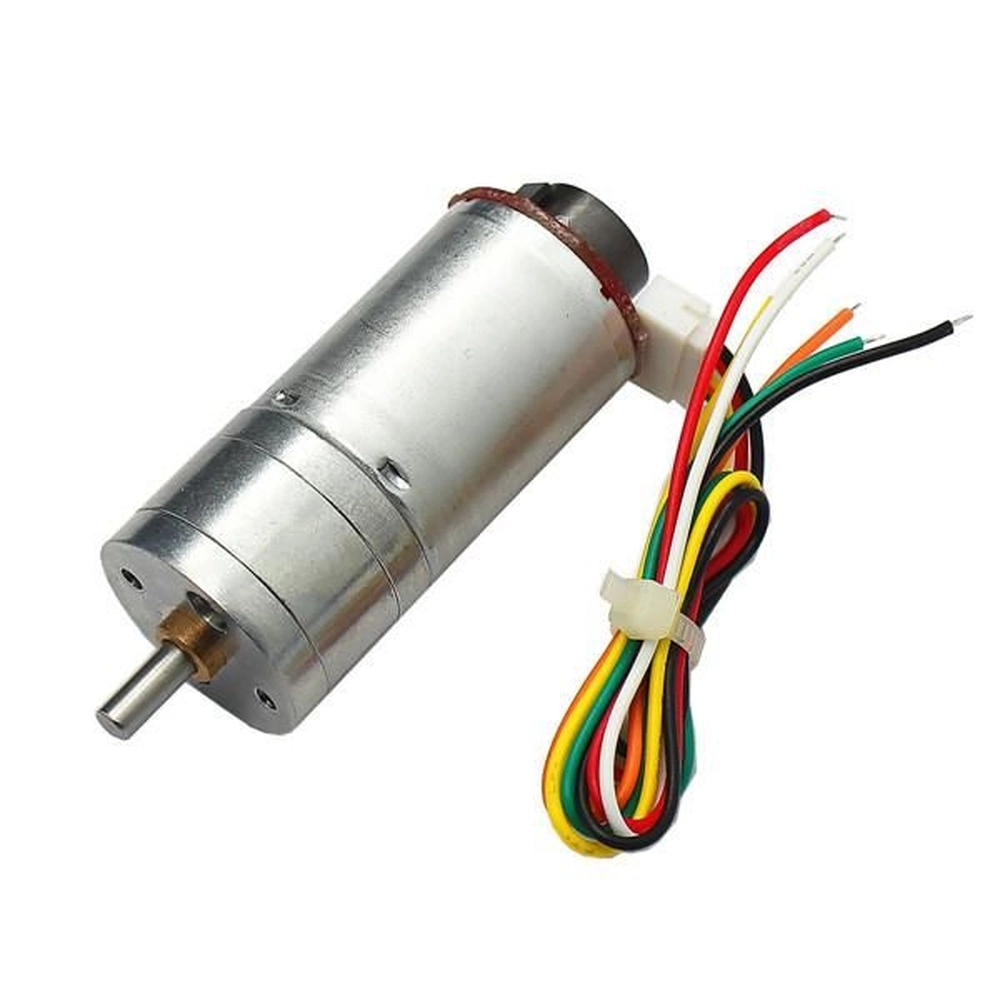
\includegraphics[width=0.7\textwidth]{figures/CHR_GM25_370}
	\caption{Motor DC 6V \cite{motor_dc_6v_encoder}}
\end{figure}

\begin{quadro}[htb]
\caption{\label{Especificacoes_motordc_6v}Especificações do motor DC 6V}
	 \begin{tabular}{|c|c|c|c|}
		\hline
		\textbf{Especificação} & \textbf{Valor} \\ \hline
		Tensão nominal & DC 6V  \\ \hline
		Velocidade sem carga  & 210RPM 0.13A  \\ \hline
		Eficiência máxima & 2,0kg.cm/170rpm/2,0W/0,60A   \\ \hline
		Poder máximo & 5,2kg.cm/110rpm/3,1W/1,10A   \\ \hline
		Torque de parada  & 10kg.cm 3.2A    \\ \hline
		Taxa de Redução do Retardador & 1:34  \\ \hline
		Resolução do salão & Razão Hall x 34,02 = 341,2PPR  \\ \hline
	\end{tabular}
	\fonte{\cite{chinhai_motor}}
\end{quadro}


\subsubsection{Driver de Motor}
Nas etapas iniciais do projeto, testou-se driver Ponte H L298N para ligar cada motor. Esse driver suporta até 2A em
operação DC \cite{datasheel_l298n}. A corrente de operação máxima do motor é de 1.1A; contudo, a corrente de parada
pode chegar a 3.2A. Além disso, o L298N também causa uma queda de tensão significativa: a uma corrente de 1A, a queda
observada chegou a até 3.2V, fazendo com que o motor não receba a tensão necessária para operar nas condições
desejadas \cite{datasheel_l298n}. As observações são compatíveis com as expectativas de faixa de operação do L298N - a
seu uso é recomendado para tensões entre 12V a 40V, em que a queda de tensão observada não seja tão significativa
relativamente. Devido à natureza da aplicação deste projeto, com o motor de 6v, a queda de tensão acaba sendo
intolerável, inviabilizando assim o uso da ponte H L298N.

Após essas considerações e observações, optou-se por um driver apropriado para uso em baixas tensões, o DRV8833
\cite{datasheel_dvr8833}.


\subsection{Controle de velocidade}

\subsubsection{Medição de velicidade do motor}

Como encoder possuí dois sinais de onda quadadra defasadas em 90º, fase A e fase B, cujos vales e picos são valores lógicos HIGH e LOW, 
e direção de rotação do motor pode ser definida pela diferença entre as fases, se fase A esta adiantada ou atrasada em relação a fase B
É possível calcular a velocidade com base nas subidas da onda quadrada de uma fase, e o valor logico da outra fase no momento da subida.
Por exemplo,  observando a fase B, toda vez em que há uma subida, se o valor da fase A for alto, então incrementar +1 em um contador, se a fase A tiver valor baixo, então incrementar -1 no contador.
Quando o valor da fase A for alto, então o motor esta rodando em um sentido,  quando o valor  for baixo, então o motor esta rodando no sentido contrário.
Medindo o valor do contador por um $\Delta_{T}$, se resulta na quantidade de pulsos por segundo.
Para converter de pulsos por segundo para RPM, basta dividir pela resolução do motor+encoder,  que é de 1:34 do motor, e 11 pulsos por rotação do encoder, o que resulta em 374,
e multiplicar por 60 para ter o resultado em rotações por minuto.

\begin{tikzpicture}[node distance=2cm]

    \node (start) [startstop] {início loop};
    \node (pro1) [process, below of=start] {ENQUANTO DELTA T};
    
    \node (in1) [io, right of=pro1, xshift= 4cm] {QUANDO FASE B = SUBIDA};
    
    \node (dec1) [decision, below of=in1, yshift=-2cm] {SE FASE A = 1};
    \node (pro1a) [process, below of=dec1, yshift= -2cm] {INCREMENTAR CONTADOR em +1};
    \node (pro1b) [process, right of=dec1, xshift= 3cm] {INCREMENTAR CONTADOR em -1};
    
    
    \node (count) [process, below of=pro1, yshift= -9cm] {CONTADOR DIVIDO POR DELTA T};
    
    \draw [arrow] (start) -- (pro1);
    \draw [arrow] (pro1) -- node[anchor=north] {sim} (in1);
    \draw [arrow] (in1) -- (dec1);
    \draw [arrow] (dec1) -- node[anchor=east] {sim} (pro1a);
    \draw [arrow] (dec1) -- node[anchor=north] {não} (pro1b);
    
    \draw [arrow] (pro1) -- node[anchor=east] {não} (count);

\end{tikzpicture}



Na implementação dessa lógica no STM32, o desafio foi a definição do $\Delta_{T}$,
Se o $\Delta_{T}$ for muito pequeno, o resultados de pulsos por segundo pode tender ao infinito, gerando valores muito altos.
Na figura \ref{fig:medidas_altas} em laranja, esta o resultado do rpm considerando o $\Delta_{T}$ como o tempo entre os ciclos do micrcontrolador.
A outra opção, foi definir um $\Delta_{T}$ fixo, definindo uma frequencia de medição pré definida, e o resultado pode ser visto em azul na figura \ref{fig:medidas_altas}
Essa outra opção de $\Delta_{T}$ resultou em um sinal que tem uma componente em alta frequência com uma amplitude até consideral.
Analisando os dois sinais no dominio da frequêcia na figura \ref{fig:frequencia_medidas_altas}, o espectro em frequência do sinal em laranja possui amplitudes muitos semelhante em todo espectro, mas o espectro do sinal em azul, fica bem claro que em altas frequencias é composto mais por ruidos
e as frequencia médias tem amplitude menor em relação as frequências baixas, o que torna mais fácil aplicar um filtro passa-baixa para reduzir as frenquências médias e altas.

A figura \autoref{passa_baixa_teste}, mostra um dos teste de filtro passa baixa, em o sinal em laranja ainda persiste esses valores tentendo ao infinito, devido a ampliture eles se tornam um pouco dificil de serem retirados.
Mas o sinal em azul acaba tendo um resultado melhor depois do filtro, muito semelhando ao sinal em laranja.
Com base nesse resultado, foi decidido seguir com o método em que o $\Delta_{T}$ é definido por uma frequência pré definida.


\begin{figure}[h]
    \centering
    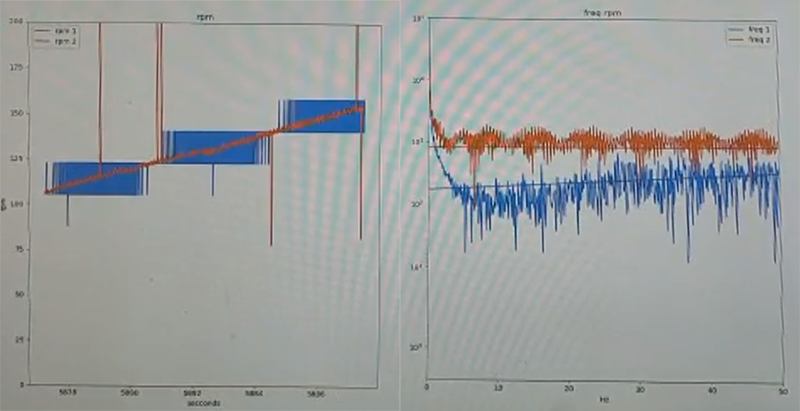
\includegraphics{figures/medidas_altas}
    \caption{Problemas com delta T muito pequeno}
    \label{fig:medidas_altas}
\end{figure}

\begin{figure}[h]
    \centering
    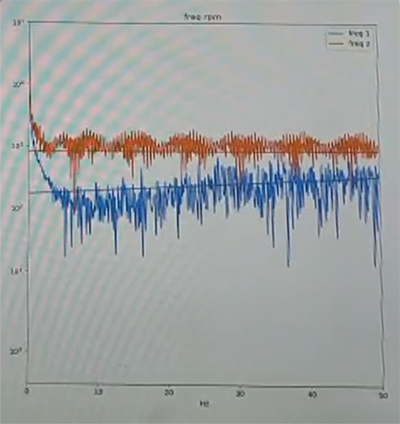
\includegraphics{figures/frequencia_medidas_altas}
    \caption{Frequências}
    \label{fig:frequencia_medidas_altas}
\end{figure}

\begin{figure}[h]
    \centering
    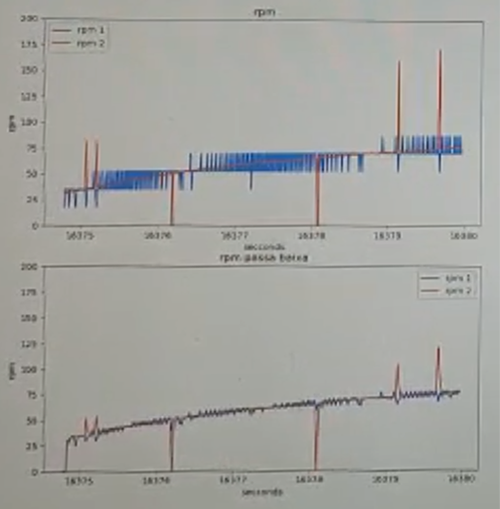
\includegraphics{figures/passa_baixa_teste}
    \caption{Passa baixa teste}
    \label{fig:passa_baixa_teste}
\end{figure}


Com o método definido, foi definido um $\Delta_{T}$ em 100hz eu um filtro passa baixa em 2hz
As imagens no anexo \autoref{att_medicao_motores}, mostra as imagens comparando o sinal original e o sinal filtrado para cada motor.
A equação \autoref{eqn:equacao_diferenca} a seguir é a equação de diferença do filtro, considerando uma amostragem de 100hz e frequência de corte em 2hz.

\begin{equation}
    \begin{split}
        y[k] = 0.0591174 \cdot u \left[ k \right] +  0.0591174 \cdot u[k - 1] + 0.88176521 \cdot y[k - 1]
    \end{split}
    \label{eqn:equacao_diferenca}
\end{equation}

\subsubsection{Curva PWM x RPM - problema da não linearidade}

Depois de definido como calcular a velocidade o próximo desafio foi lidar com a não linearidade entre o PWM e o resultado medido em RPM.
Como pode ser visto na figura \autoref{grafico_pwm_x_rpm}, na comparação entre o valor do PWM e o RPM no tempo.

\begin{figure}[htb]
	\centering
	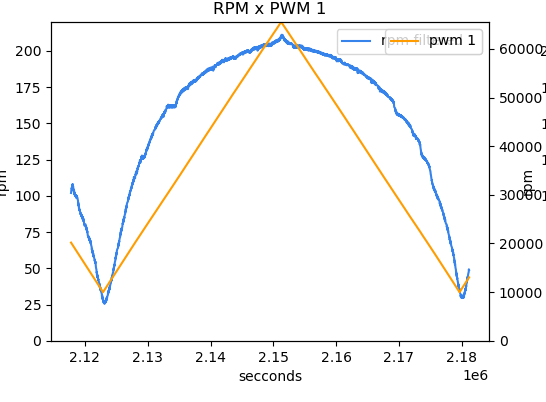
\includegraphics{figures/pwm_x_rpm}
	\caption{Curva PWM e RPM no tempo}
	\label{fig:grafico_pwm_x_rpm}
\end{figure}

Considerando essa não linearidade, foram realizadas 15k medições em PWM vs RPM para definir uma equação que pudesse relacionar o PWM com o RPM.
Como pode ser observado na figura  \autoref{medicao_pwm_x_rpm_dados_brutos}, os resultados possuem uma tendência, mas possuem alguns pontos fora da curta.
devido ao esses ruídos nas medições ss dados foram tratatos para obter valores médios dos resultados usando python,
o código pode ser visto no anexo \autoref{att_limpeza_python}.

\begin{figure}[htb]
	\centering
	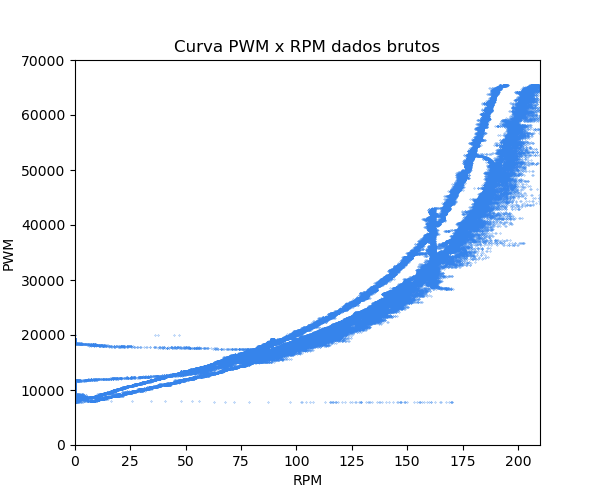
\includegraphics{figures/curva_pwm_x_rpm_dados_brutos}
	\caption{Curva PWM x RPM dados brutos}
	\label{fig:medicao_pwm_x_rpm_dados_brutos}
\end{figure}


O resultado da limpeza dos dados pode ser vizualizado na figura \autoref{medicao_pwm_x_rpm_dados_medios}.
Após a limpeza dos dados, os dados foram importados para o matlab, anexo \autoref{att_matlab},
para obter um polinômio que possa definir a curva, o polinômio resultante é a equação \ref{eqn:polimonio_rpm}, e a figura \autoref{curva_ajustada} representa a curva ajustada.
A equação do polinômio foi inserida no código do micrcontrolador, foi testado definir um RPM de 150, e a tabela \autoref{medicao_motores} trás uma amostra dos resultados dos RPMs de cada motor.
Com essa equação é mais fácil definir um comportamento linear, facilitando a aplicação de um controle PDI.

\begin{equation}
    \begin{split}
        0.0001131x^{4} + -0.03064x^{3} + 2.993x^{2} + -1.257x + 9017
    \end{split}
    \label{eqn:polimonio_rpm}
\end{equation}

\begin{figure}[htb]
	\centering
	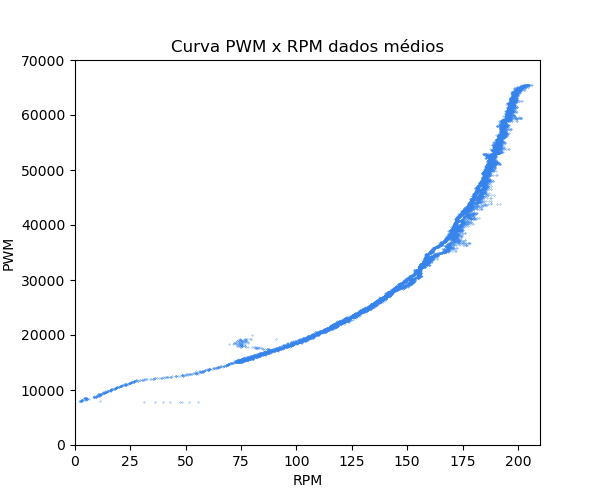
\includegraphics{figures/curva_pwm_x_rpm_dados_medios}
	\caption{Curva PWM x RPM dados médios}
	\label{fig:medicao_pwm_x_rpm_dados_medios}
\end{figure}

\begin{figure}[htb]
	\centering
	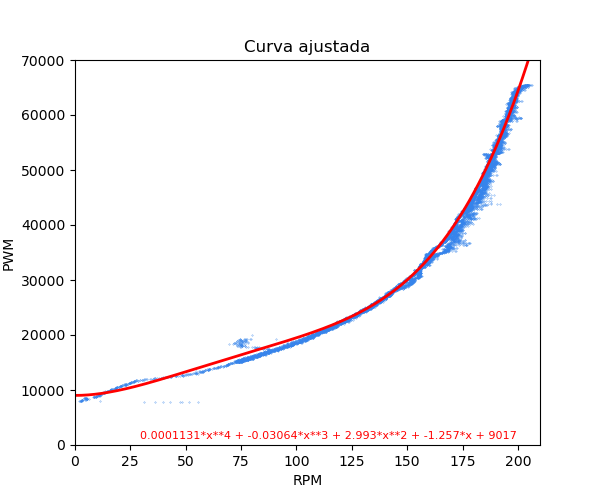
\includegraphics{figures/curva_ajustada}
	\caption{Curva ajustada}
	\label{fig:curva_ajustada}
\end{figure}



\begin{quadro}[htb]
	\caption{\label{medicao_motores}Medição rpms motores}
	 \begin{tabular}{|c|c|c|c|c|}
		\hline
		\textbf{$Tempo_{seg}$} & \textbf{$RPM_{definido}$} & \textbf{$RPM_{real_{1}}$} & \textbf{$RPM_{real_{2}}$} & \textbf{$RPM_{real_{3}}$} \\ \hline
		52.954 & 150.00  & 141.03 & 162.69 & 149.82 \\ \hline
		52.954 & 150.00  & 141.43 & 162.43 & 149.18 \\ \hline
		53.000 & 150.00  & 140.83 & 162.19 & 148.61 \\ \hline
		53.000 & 150.00  & 140.30 & 161.98 & 149.06 \\ \hline
		53.000 & 150.00  & 140.79 & 161.80 & 149.46 \\ \hline
		53.000 & 150.00  & 141.21 & 161.64 & 148.86 \\ \hline
		53.046 & 150.00  & 141.59 & 161.49 & 149.28 \\ \hline
		53.046 & 150.00  & 141.92 & 161.37 & 149.65 \\ \hline
		53.046 & 150.00  & 141.26 & 161.25 & 149.02 \\ \hline
		53.046 & 150.00  & 140.68 & 162.11 & 148.48 \\ \hline
		53.046 & 150.00  & 141.12 & 162.86 & 148.94 \\ \hline
		53.092 & 150.00  & 141.51 & 162.57 & 149.35 \\ \hline
		53.092 & 150.00  & 141.85 & 162.32 & 148.76 \\ \hline
		53.092 & 150.00  & 141.20 & 162.09 & 149.19 \\ \hline
		53.092 & 150.00  & 140.63 & 161.90 & 149.57 \\ \hline
	\end{tabular}
\end{quadro}


\subsection{Implementação da medição de rpm e filtro passa baixa no microcontrolador}

Para medir a velocidade de um motor DC com base no encoder, foi necessário realizar a leitura das subidas dos calores de LOW para HIGH de uma das fases do enconder, e comparar com outra Fase
Para isso usamos o sistema de interrupção do microcontrolador.
Exemplo do trecho de código que realiza a leitura dos valores do encoder, e registra em um contador a quantidade de pulsos de uma fase.


\lstset{language=C}
\begin{lstlisting}
long prevTime = 0;
long currTime = micros();
volatile int pos_i_1 = 0;
int prevPosition_1 = 0;
void setup() {
    motorsSetupPins(); encodersSetupPins();
    attachInterrupt(digitalPinToInterrupt(PB0), readEncoder1, RISING);
}
void loop() {
	int currPosition_1 = 0;
    ATOMIC_BLOCK(ATOMIC_RESTORESTATE){currPosition_1 = pos_i_1;};
    prevPosition_1 = currPosition_1;
}

void readEncoder1(){ 
    int b = digitalRead(PB1);
    if(b>0){pos_i_1++;}
    else {pos_i_1--;}
}
\end{lstlisting}


Após obtendo os a quantidade de pulsos é possivel calcular a taxa de pulsos por segundo, usando o diferencial da velocidade no dominio discreto, $\Delta$p/$\Delta$t.

\lstset{language=C}
\begin{lstlisting}
#define HALL_RESOLUTION 374
long prevTime = 0;
long currTime = micros();
volatile int pos_i_1 = 0;
int prevPosition_1 = 0;
float direction_angle = 90;
void setup() {
    motorsSetupPins();
    encodersSetupPins();
    attachInterrupt(digitalPinToInterrupt(PB0), readEncoder1, RISING);  
}
void loop() {
	currTime = micros();
	int currPosition_1 = 0;
	ATOMIC_BLOCK(ATOMIC_RESTORESTATE){currPosition_1 = pos_i_1;};
	float rpm1 = calc_rpm(currTime, prevTime, currPosition_1, prevPosition_1);
	prevPosition_1 = currPosition_1;
	prevPosition_3 = currPosition_3;
	prevTime = currTime;
}
void readEncoder1(){ 
    int b = digitalRead(PB1);
    if(b>0){pos_i_1++;}
    else {pos_i_1--;}
}
float calc_rpm(long currT, long prevT, int pos, int posPrev){
    float deltaT = ((float) (currT-prevT))/1.0e6;
    float pulse_per_seconds = (pos - posPrev)/deltaT;
    float rpm = 60*pulse_per_seconds/HALL_RESOLUTION;
    return rpm;
}
\end{lstlisting}


Porém calcular velocidade a cada ciclo do micrcontrolador acaba registrando valores de tempo muito pequenos, fazendo a velocidade tender ao infinito
A solução foi estabelecer uma amostragem do registro da velocidade, porem a amostragem adiciona um ruido com frequências maiories que do sinal original e de amplitude definida.
Para retirar essas frequência do sinal, o filtro passa baixa foi implementado no código.


\lstset{language=C}
\begin{lstlisting}
#define HALL_RESOLUTION 374
#define DT_TIME_SAMPLE_RATE_ENCODER 10 // encoder position reading update rate
int nextChangeSampleRate  = (millis() + DT_TIME_SAMPLE_RATE_ENCODER);
long prevTime = 0;
long currTime = micros();
volatile int pos_i_1 = 0;
int prevPosition_1 = 0;
float filterRpm_1 = 0;
float prevRpm_1 = 0;
void setup() {
    encodersSetupPins();
    attachInterrupt(digitalPinToInterrupt(PB0), readEncoder1, RISING);   
}

void loop() {
    if (millis()>=nextChangeSampleRate){
        currTime = micros();
        int currPosition_1 = 0;
        ATOMIC_BLOCK(ATOMIC_RESTORESTATE){currPosition_1 = pos_i_1;};
        float rpm1 = calc_rpm(currTime, prevTime, currPosition_1, prevPosition_1);
        filterRpm_1 = low_pass_filter_first_order(rpm1, prevRpm_1, filterRpm_1);
        prevPosition_1 = currPosition_1;
        prevRpm_1 = rpm1;
        prevTime = currTime;
        nextChangeSampleRate = millis() + DT_TIME_SAMPLE_RATE_ENCODER;
    }
}
void readEncoder1(){ 
    int b = digitalRead(PB1);
    if(b>0){pos_i_1++;}
    else {pos_i_1--;}
}
float calc_rpm(long currT, long prevT, int pos, int posPrev){
    float deltaT = ((float) (currT-prevT))/1.0e6;
    float pulse_per_seconds = (pos - posPrev)/deltaT;
    float rpm = 60*pulse_per_seconds/HALL_RESOLUTION;
    return rpm;
}
float low_pass_filter_first_order(float currRpm, float prevRpm, float prevFilterRpm){
    float posFilterRpm = 0.881765*prevFilterRpm + 0.0591174*currRpm + 0.0591174*prevRpm;
    return posFilterRpm;
}
\end{lstlisting}

\subsection{Motores de passo}

\lipsum[1]




%https://www.aarohies.com/what-is-the-difference-between-pmdc-bldc-and-pmsm-motor/
%https://www.monolithicpower.com/en/learning/resources/brushless-vs-brushed-dc-motors
%https://techweb.rohm.com/product/motor/brushed-motor/209/